\documentclass[nofootinbib,amssymb,amsmath]{revtex4}
\usepackage{mathtools}
\usepackage{amsthm}
\usepackage{algorithm}
\usepackage{algpseudocode}
\usepackage{lmodern}
\usepackage{graphicx}
\usepackage{color}
\usepackage{bm}

%Put an averaged random variable between brackets
\newcommand{\ave}[1]{\left\langle #1 \right\rangle}

\newcommand{\vzero}{{\bf 0}}
\newcommand{\vI}{{\bf I}}
\newcommand{\vb}{{\bf b}}
\newcommand{\vd}{{\bf d}}
\newcommand{\vf}{{\bf f}}
\newcommand{\vc}{{\bf c}}
\newcommand{\vv}{{\bf v}}
\newcommand{\vz}{{\bf z}}
\newcommand{\vn}{{\bf n}}
\newcommand{\vm}{{\bf m}}
\newcommand{\vG}{{\bf G}}
\newcommand{\vQ}{{\bf Q}}
\newcommand{\vM}{{\bf M}}
\newcommand{\vW}{{\bf W}}
\newcommand{\vX}{{\bf X}}
\newcommand{\vPsi}{{\bf \Psi}}
\newcommand{\vSigma}{{\bf \Sigma}}
\newcommand{\vlambda}{{\bf \lambda}}
\newcommand{\vpi}{{\bf \pi}}
\newcommand{\valpha}{{\bm{\alpha}}}
\newcommand{\vbeta}{{\bm{\beta}}}
\newcommand{\vomega}{{\bm{\omega}}}
\newcommand{\vLambda}{{\bf \Lambda}}
\newcommand{\vA}{{\bf A}}

\newcommand{\code}[1]{\texttt{#1}}

\newtheorem{lemma}{Lemma}
\newtheorem{corollary}{Corollary}

\def\SL#1{{\color [rgb]{0,0,0.8} [SL: #1]}}
\def\DB#1{{\color [rgb]{0,0.8,0} [DB: #1]}}

\newcommand{\HOM}{$\mathsf{Hom}$}
\newcommand{\HET}{$\mathsf{Het}$}
\newcommand{\REF}{$\mathsf{Ref}$}
\newcommand{\epss}{\varepsilon}

\begin{document}

\title{Mathematical Notes on Mutect}
\author{David Benjamin}
\email{davidben@broadinstitute.org}
\affiliation{Broad Institute, 75 Ames Street, Cambridge, MA 02142}
\author{Takuto Sato}
\email{tsato@broadinstitute.org}
\affiliation{Broad Institute, 75 Ames Street, Cambridge, MA 02142}

\date{\today}

\maketitle

\section{Somatic Likelihoods Model}\label{introduction}

We have a set of potential somatic alleles and read-allele likelihoods $\ell_{ra} \equiv P({\rm read~}r|{\rm allele~}a)$.  We don't know which alleles are real somatic alleles and so we must compute, for each subset $\mathbb{A}$ of alleles, the likelihood that the reads come from $\mathbb{A}$.  A simple model for this likelihood is as follows: each read $r$ is associated with a latent indicator vector $\vz_r$ with one-hot encoding $z_{ra} = 1$ iff read $r$ came from allele $a \in \mathbb{A}$.  The conditional probability of the reads $\mathbb{R}$ given their allele assignments is
\begin{equation}
P( \mathbb{R} | \vz, \mathbb{A}) = \prod_{r \in \mathbb{R}} \prod_a \ell_{ra}^{z_{ra}}.
\end{equation}
The alleles are not equally likely because there is a latent vector $\vf$ of allele fractions -- $f_a$ is the allele fraction of allele $a$.  Since the components of $\vf$ sum to one it is a categorical distribution and can be given a Dirichlet prior,
\begin{equation}
P(\vf) = {\rm Dir}(\vf | \valpha).
\end{equation}
Then $f_a$ is the prior probability that a read comes from allele $a$ and thus the conditional probability of the indicators $\vz$ given the allele fractions $\vf$ is
\begin{equation}
P(\vz | \vf) = \prod_r \prod_a f_a^{z_{ra}}.
\end{equation}
The full-model likelihood is therefore
\begin{equation}
\mathbb{L}(\mathbb{A}) = P(\mathbb{R}, \vz, \vf | \mathbb{A}) = {\rm Dir}(\vf | \valpha) \prod_a  \prod_r \left( f_a \ell_{ra}\right)^{z_{ra}}.
\label{full_likelihood}
\end{equation}
And the marginalized likelihood of $\mathbb{A}$, that is, the model evidence for allele subset $\mathbb{A}$, is
\begin{equation}
P(\mathbb{R} | \mathbb{A}) = \sum_\vz \int d \vf \, {\rm Dir}(\vf | \valpha) \prod_a  \prod_r \left( f_a \ell_{ra}\right)^{z_{ra}},
\label{evidence}
\end{equation}
where the integral is over the probability simplex $\sum_a f_a = 1$.

The integral over $\vf$ is the normalization constant of a Dirichlet distribution and as such we can simply look up its formula.  However, the sum over all values of $\vz$ for all reads has exponentially many terms.  We will get around this difficulty by handling $\vz$ with a mean-field approximation in which we factorize the likelihood as $\mathbb{L} \approx q(\vz) q(\vf)$.  This approximation is exact in two limits: first, if there are many reads, each allele is associated with many reads and therefore the Law of Large Numbers causes $\vf$ and $\vz$ to become uncorrelated.  Second, if the allele assignments of reads are obvious $\vz_r$ is effectively not a random variable at all (there is no uncertainty as to which of component is non-zero) and also becomes uncorrelated with $\vf$.

In the variational Bayesian mean-field formalism the value of $\vf$ that $\vz$ ``sees'' is the expectation of $\log \mathbb{L}$ with respect to $q(\vf)$ and vice versa.  That is,
\begin{equation}
q(\vf) \propto {\rm Dir}(\vf | \valpha) \prod_a  \prod_r f_a^{\bar{z}_{ra}} \propto {\rm Dir}(\vf | \valpha + \sum_r \bar{\vz}_r),
\label{qf}
\end{equation}
where $\bar{z}_{ra} \equiv E_q \left[ z_{ra} \right]$, and
\begin{equation}
q(\vz_r) = \prod_a \left( \tilde{f}_a \ell_{ra}\right)^{z_{ra}}, \tilde{f}_a = \exp E[\ln f_a]
\end{equation}
Because $q(\vz)$ is categorical and $q(\vf)$ is Dirichlet\footnote{Note that we didn't \textit{impose} this in any way.  It simply falls out of the mean field equations.} the necessary mean fields are easily obtained and we have
\begin{equation}
\bar{z}_{ra} = \frac{\tilde{f}_a \ell_{ra}}{\sum_{a^\prime} \tilde{f}_{a^\prime} \ell_{ra^\prime}}
\label{z_mean_field}
\end{equation}
and
\begin{equation}
\ln \tilde{f}_a = \psi(\alpha_a + \sum_r \bar{z}_{ra}) - \psi(\sum_{a^\prime} \alpha_{a^\prime} + N)
\label{f_mean_field}
\end{equation}
where $\psi$ is the digamma function and $N$ is the number of reads.  To obtain $q(\vz)$ and $q(\vf)$ we iterate Equations \ref{z_mean_field} and \ref{f_mean_field} until convergence.  A very reasonable initialization is to set $\bar{z}_{ra} = 1$ if $a$ is the most likely allele for read $r$, 0 otherwise.  Having obtained the mean field of $\vz$, we would like to plug it into Eq \ref{evidence}.  We can't do this directly, of course, because Eq \ref{evidence} says nothing about our mean field factorization.  Rather, we need the variational approximation (Bishop's Eq 10.3) to the model evidence, which is
\begin{align}
\ln P(\mathbb{R} | \mathbb{A}) \approx& \sum_{\vz} \int d \vf q(\vz) q(\vf) \left[ \ln P(\mathbb{R}, \vz, \vf | \mathbb{A}) - \ln q(\vz) - \ln q(\vf) \right] \\
=& E_q \left[ \ln P(\mathbb{R}, \vz, \vf | \mathbb{A}) \right] - E_q \left[ \ln q(\vz) \right] - E_q \left[ \ln q(\vf) \right]. \label{lagrangian}
\end{align}
Before we proceed, let's introduce some notation.  First, from Eq \ref{qf} the posterior $q(\vf)$ is
\begin{equation}
q(\vf) = {\rm Dir}(\vf | \vbeta), \quad \vbeta = \valpha + \sum_r \bar{\vz}_r.
\end{equation}
Second, let's define the log normalization constant of a Dirichlet distribution as $g$ so that
\begin{equation}
\ln {\rm Dir}(\vf | \vomega) = g(\vomega) + \sum_a (\omega_a - 1) \ln f_a, \quad g(\vomega) = \ln \Gamma(\sum_a \omega_a) - \sum_a \ln \Gamma(\omega_a).
\end{equation}
Finally, define the Dirichlet mean log (aka ``that digamma stuff") as $h$:
\begin{equation}
E_{\rm Dir(\vf | \vomega)} \left[ \ln f_a \right] = \psi(\omega_a) - \psi(\sum_{a^\prime} \omega_{a^\prime}) \equiv h_a(\vomega).
\end{equation}

The log of Eq \ref{full_likelihood} is
\begin{equation}
\ln P(\mathbb{R}, \vz, \vf | \mathbb{A}) = g(\valpha) + \sum_a (\alpha_a - 1) \ln f_a + \sum_{ra} z_{ra} (\ln f_a + \ln \ell_{ra}).
\end{equation}
and thus the first term in Eq \ref{lagrangian} is
\begin{align}
E_q \left[ \ln P(\mathbb{R}, \vz, \vf | \mathbb{A}) \right] =& g(\valpha) + \sum_a (\alpha_a - 1) h_a(\vbeta) + \sum_{ra}\bar{z}_{ra} \left( h_a(\vbeta) + \ln \ell_{ra} \right) \\
=& g(\valpha) + \sum_a (\beta_a - 1) h_a(\vbeta) + \sum_{ra}\bar{z}_{ra} \ln \ell_{ra}, \label{first_term}
\end{align}
where we used the relationship $\vbeta = \valpha + \sum_r \bar{\vz}_r$.

The second term in Eq \ref{lagrangian} is
\begin{align}
- E_q \left[ \ln q(\vz) \right] = - \sum_{ra} \bar{z}_{ra} \ln \bar{z}_{ra} \label{second_term}.
\end{align}

The third term in Eq \ref{lagrangian} is
\begin{align}
- E_q \left[ \ln q(\vf) \right] = -g(\vbeta) - \sum_a (\beta_a - 1) E_q [\ln f_a] = -g(\vbeta) - \sum_a (\beta_a - 1) h_a(\vbeta) \label{third_term}.
\end{align}

Adding Eqs \ref{first_term}, \ref{second_term}, and \ref{third_term} and noting the cancellation between parts of Eqs \ref{first_term} and \ref{third_term} we obtain
\begin{equation}
\ln P(\mathbb{R} | \mathbb{A}) \approx g(\valpha) - g(\vbeta) +  \sum_{ra} \bar{z}_{ra} \left( \ln \ell_{ra} - \ln \bar{z}_{ra} \right).
\end{equation}

We now have the model evidence for allele subset $\mathbb{A}$.  This lets us choose which alleles are true somatic variants.  It also lets us make calls on somatic loss of heterozygosity events.  Furthermore, instead of reporting max-likelihood allele fractions as before, we may emit the parameters of the Dirichlet posterior $q(\vf)$, which encode both the maximum likelihood allele fractions and their uncertainty.

\section{Strand Artifact Model}
\begin{figure}
\centering
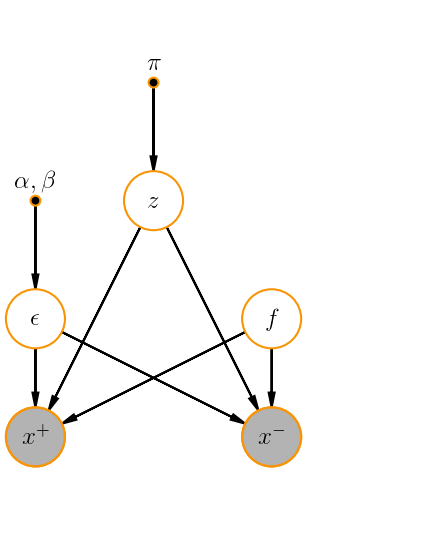
\includegraphics[width=0.3\textwidth]{strand_artifact_pgm.png}
\caption{\label{fig:frog}The probabilistic graphical model}
\end{figure}

\begin{itemize}
	\item $\vz$ is a latent random variable having a 1-of-K representation. For each variant locus, $\vz$ encodes the presence of strand artifact in forward reads ($[1, 0, 0]$), artifact in reverse reads ($[0, 1, 0]$), or no artifact ($[0, 0, 1]$)
	\item $f \sim \text{Unif}(0, 1)$ is a prior distribution over alt allele fraction $f$
	\item $\epsilon \sim \text{Beta}(\alpha, \beta)$ is a prior distribution over the error probability on a read on the artifact strand. For instance, if we have strand artifact on the reverse strand (i.e. $z = [0, 1, 0]$), $\epsilon$ is the probability that the sequencer reads a ref allele on a reverse read as alt
	\item $x^+ | f, \epsilon, z$ is the number of forward reads with the alt allele. It's a mixture of binomials, defined as follows:
	\begin{equation}
	x^+ | f, \epsilon, z \sim
		\begin{cases}
			\text{Bin} (n^+, f + \epsilon(1-f)) & z = \mathrm{Art+}\\
			 \text{Bin} (n^+, f) 			& z = \mathrm{Art-} \\
			 \text{Bin} (n^+, f)			& z = \mathrm{noArt}
		\end{cases}
	\end{equation}
\end{itemize}



We compute the conditional distributions of $x^-$  analogously.

Having observed the read counts in the forward and reverse directions, we can compute the posterior probabilities of the latent variable $z$.  Below we derive the unnormalized posterior probability of strand artifact in forward reads ($z = art+$), given that we observed $x^+$ forward alt reads and $x^-$ reverse alt reads. We use a shorthand $z_0$ to denote $z=art+$ for conciseness. 

First we will derive the likelihood $p(x^+, x^-, f, \epsilon | z_0)$
\begin{align}
p(x^+, x^- | z_0)  &= \iint_{f, \epsilon}  p(x^+, x^-, f, \epsilon | z_0) \,df\,d\epsilon \\
			  &= \iint_{f, \epsilon}  p(f) p(\epsilon) p(x^+, x^- | z_0, f, \epsilon) \,df\,d\epsilon \\
			  &= \iint_{f, \epsilon}  p(f) p(\epsilon) p(x^+ | z_0, f, \epsilon) p(x^- | z_0, f, \epsilon) \,df\,d\epsilon \\
			  &= \iint_{f, \epsilon}  p(\epsilon) p(x^+ | z_0, f, \epsilon) p(x^- | z_0, f, \epsilon) \,df\,d\epsilon \label{watershed} \\
			  &= \iint_{f, \epsilon}  \mathrm{Beta}(\epsilon|\alpha, \beta) \mathrm{Bin}(x^+ | f + \epsilon(1-f), n^+) \mathrm{Bin}(x^- | f, n^-) \,df\,d\epsilon
\end{align}

The posterior probability of strand artifact in forward reads is therefore

\begin{align}
p(z_0 |x^+, x^-) & \propto p(z_0) p(x^+, x^- | z_0) \\
			 & = p(z_0) \iint_{f, \epsilon}  \mathrm{Beta}(\epsilon|\alpha, \beta) \mathrm{Bin}(x^+ | f + \epsilon(1-f), n^+) \mathrm{Bin}(x^- | f, n^-) \,df\,d\epsilon
\end{align}

The derivation for the probability of strand artifact on reverse strand is analogous.

For the case of no strand artifact, the derivation of likelihoods is identical up to (\ref{watershed}). Here we can simply the equation to a single integral over $f$ because the conditional probabilities of $x^+$ and $x^-$ do not depend on $\epsilon$. We use a shorthand $z_2$ for $z=\mathrm{noArt}$

\begin{align}
p(x^+, x^- | z_2)  &= \iint_{f, \epsilon}  p(\epsilon) p(x^+ | z_2, f, \epsilon) p(x^- | z_2, f, \epsilon) \,df\,d\epsilon \nonumber \\
			  &= \int_{f}  p(x^+ | z_2, f) p(x^- | z_2, f) \,df \int_{\epsilon}  p(\epsilon) d\epsilon \\
			  &= \int_{f}  \mathrm{Bin}(x^+ | f, n^+) \mathrm{Bin}(x^- | f, n^-) \,df
\end{align}

And the posterior probability is

\begin{align}
p(z_2 |x^+, x^-) & \propto p(z_2) p(x^+, x^- | z_2) \\
                         & = p(z_2) \int_{f}  \mathrm{Bin}(x^+ | f, n^+) \mathrm{Bin}(x^- | f, n^-) \,df
\end{align}


\section{Germline Filter}\label{germline-filter}
Suppose we have detected an allele such that its (somatic) likelihood in the tumor is $\ell_t$ and its (diploid) likelihood in the normal is $\ell_n$.  By convention, both of these are relative to a likelihood of $1$ for the allele \textit{not} to be found.  If we have no matched normal, $\ell_n = 1$.  Suppose we also have the population allele frequency $f$ of this allele.  Then the prior probability for the normal to be heterozygous or homozygous alt for the allele is $2f(1-f) + f^2$ and the prior probability for the normal genotype not to contain the allele is $(1-f)^2$.  Finally, suppose that the prior for this allele to arise as a somatic variant is $\pi$.

We can determine the posterior probability that the variant exists in the normal genotype by calculating the unnormalized probabilities of four possibilities:
\begin{enumerate}
\item The variant exists is both the normal and the tumor samples.  This has unnormalized probability $\left(2f(1-f) + f^2 \right) \ell_n \ell_t (1 - \pi)$.
\item The variant exists in the tumor but not the normal.  This has unnormalized probability $(1-f)^2 \ell_t \pi$.
\item The variant exists in neither the tumor nor the normal.  This has unnormalized probability $(1-f)^2 (1 - \pi)$.
\item The variants exists in the normal but not the tumor.  This is biologically very unlikely.  Furthermore, if it \textit{did} occur we wouldn't care about filtering the variant as a germline event because we wouldn't call it as a somatic event.  Thus we neglect this possibility.
\end{enumerate}

Normalizing, we obtain the following posterior probability that an allele is a germline variant:
\begin{equation}
P({\rm germline}) = \frac{(1)}{(1) + (2) + (3)} = \frac{\left(2f(1-f) + f^2 \right) \ell_n \ell_t (1 - \pi)}{\left(2f(1-f) + f^2 \right) \ell_n \ell_t (1 - \pi) + (1-f)^2 \ell_t \pi + (1-f)^2 (1 - \pi)}.
\end{equation}

To filter, we set a threshold on this posterior probability.

\end{document}